\
\
\
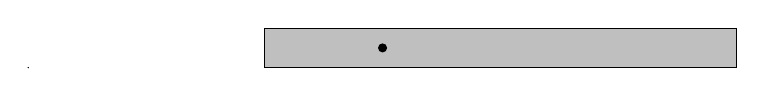
\begin{tikzpicture}
\draw (0,0) circle (0.00001cm);
\filldraw[fill = lightgray, draw = black] (3,0) -- (9,0) -- (9,0.5) -- (3,0.5) -- (3,0); 
\filldraw (4.5,0.25) circle (0.05cm);
\end{tikzpicture}
\newline
\newline
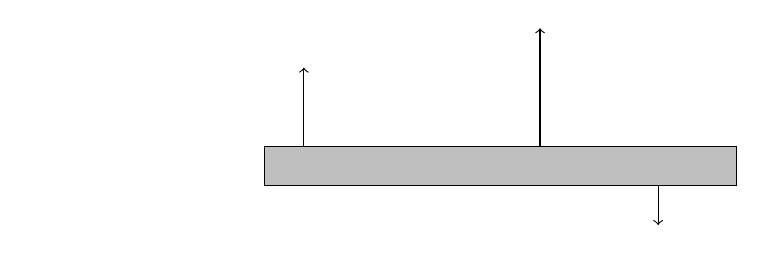
\begin{tikzpicture}
\draw (0,0) circle (0.000001cm);
\filldraw[fill = lightgray, draw = black] (3,0) -- (9,0) -- (9,0.5) -- (3,0.5) -- (3,0); 
\draw[->] (3.5,0.5) -- (3.5,1.5);
\draw[->] (6.5,0.5) -- (6.5,2);
\draw[->] (8,0) -- (8,-0.5);
\end{tikzpicture}
\newline
\newline
Torque is a relatively confusing topic because there are so few examples that we can see and relate it too. People move stuff and pick stuff up all the time, but very rarely do we rotate things at constant rates. Additionally, torque is a funny concept because it will vary with the point that we define it about. 

The first example can be the classic example of a rod pinned down at its end that we are trying to rotate around. We imagine that the axis of rotation is coming out of the page.  We know from our physical intuition that if we pull in the direction of the rod, the rot will not rotate, that would not make any sense. However, it is not necessarily clear that if we, for example, push a rod at a $45^o$ angle, that it will rotate any less fast than if we are to push a rod at a $90^o$ angle. However, tests have conclusively shown that the speed of acceleration of a rod given a certain pushing force, will vary with the $\sin$ of the angle between the force on the rod and the distance from the axis of rotation of the rod to the point where the force is being applied. It is also clear that if we are trying to rotate a rod, if we push directly at the point, or very near the point at which the object is being rotated, it will be tough to rotate the rod. It is not necessarily clear, however, that the farther along the rod that we push, the faster the rod will rotate given a certain constant force and angle of pushing against the rod. We can sum up these things that we see in nature in a relatively simple formula. This is that torque, denoted as \begin{equation}\vec{\tau}= \vec{r} \times \vec{F}\end{equation} Torque is the rotational analog of force, so we need to have a formula for torque analogous to $$\vec{F}=m\vec{a}$$ This is simple enough to create because $I$ is the rotational equivalent to $m$ and $\alpha$ is the rotational equivalent to $a$. So We have that $$\tau=I \alpha$$ Essentially this means that the torque being applied to an object is equal to its moment of inertia times the rate at which the object is accelerating angularly. Similar to angular momentum, we can see that torque is a vector, and its magnitude is equal to $$rp\sin\left(\theta \right)$$ where $\theta$ is the angle between the vector from the axis of rotation of the object and the direction of the force on the object. We can think about this with the example of two opposing forces operating on the same sides of a rod. It should be natural that if the forces are equal to each other, then the object will not rotate. We can verify this using the idea of torque and using the right-hand rule. Again, we can assume the object will rotate about its center so the $\vec{r}$ vector will be defined from the center of the rod to the edge of the rod, where the force is being applied. Torque is a difficult concept because often the axis of rotation may not be known, may be changing with time, or the force may be changing with time. This occurs when the object is not necessarily bolted to anything and maybe moving linearly in addition to rotationally, we will not see too many examples of this but as you might be able to tell, it can be tough to deal with these situations.